\documentclass[11pt]{article}
\usepackage[margin=1in]{geometry}
\usepackage{amsmath,amssymb}
\usepackage{tikz}
\usetikzlibrary{arrows.meta,positioning,calc}
\usepackage{pgfplots}
\usepackage{float}
\pgfplotsset{compat=1.18}
\usepackage[colorlinks=true,linkcolor=blue!50!black]{hyperref}
\colorlet{cmid}{blue!65!cyan!80!black}
\colorlet{cout}{orange!85!black}
\pgfplotsset{every axis/.append style={label style={font=\small}, tick label style={font=\footnotesize}}}

\title{Visualizing the balanced-split pivot}
\author{Companion to \emph{One more fold per node}, Sec.~II.A--II.C}
\date{}

\begin{document}
\maketitle

\noindent All figures use one Haar-random four-qubit target ($n=4$, so $D=2^{n-1}=8$), computed
with \texttt{stage2/foldzxz\_opt.py}. The middle half of the sorted list is drawn in
\textcolor{cmid}{blue} and the outer quarters in \textcolor{cout}{orange} throughout.

\section*{1. What we want: one zero angle}

After demultiplexing, the left-side multiplexor is a Gray-code sequence of $D$ rotations
$R_z(\varphi_k)$ separated by CX gates, with angles $\boldsymbol\varphi=\tfrac1D H_D\boldsymbol\theta$
given by the Walsh--Hadamard transform of the multiplexor angles $\boldsymbol\theta$, which are the
eigenphases of $C(g)$. The last rotation, between the final two CX gates, has angle
\[
\varphi=\tfrac1D\,\mathbf h^{\mathsf T}\boldsymbol\theta,\qquad h_j=(-1)^{j_{n-2}},
\]
so it compares the sum of the angles on the half $j_{n-2}=0$ with the sum on $j_{n-2}=1$. If the two
sums agree, $\varphi=0$, the two CX gates become adjacent, and both merge into the central factor.
We are free to decide which eigenphases go on which half (and to shift each by $2\pi$); the
question is only whether some assignment balances. Figure~\ref{fig:pipeline} shows how the pivot
$g=R_z(\alpha)R_y(\beta)$ controls this, and where the two one-dimensional searches enter.

\begin{figure}[H]
\centering
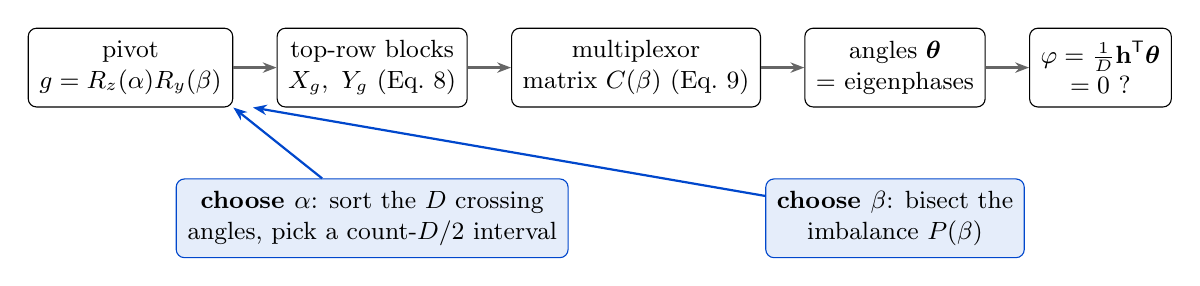
\begin{tikzpicture}[node distance=0.55cm,
  box/.style={draw, rounded corners=3pt, align=center, font=\small, inner sep=4pt, minimum height=1cm},
  srch/.style={box, fill=cmid!10, draw=cmid},
  arr/.style={-{Stealth[length=5pt]}, black!60, thick}]
\node[box] (g) {pivot\\ $g=R_z(\alpha)R_y(\beta)$};
\node[box, right=of g] (xy) {top-row blocks\\ $X_g,\ Y_g$ (Eq.~8)};
\node[box, right=of xy] (c) {multiplexor\\ matrix $C(\beta)$ (Eq.~9)};
\node[box, right=of c] (th) {angles $\boldsymbol\theta$\\ $=$ eigenphases};
\node[box, right=of th] (phi) {$\varphi=\tfrac1D\mathbf h^{\mathsf T}\boldsymbol\theta$\\ $=0$ ?};
\draw[arr] (g)--(xy); \draw[arr] (xy)--(c); \draw[arr] (c)--(th); \draw[arr] (th)--(phi);
\node[srch, below=0.9cm of xy] (sa) {\textbf{choose $\alpha$}: sort the $D$ crossing\\ angles, pick a count-$D/2$ interval};
\node[srch, below=0.9cm of th] (sb) {\textbf{choose $\beta$}: bisect the\\ imbalance $P(\beta)$};
\draw[arr, cmid] (sa) -- (g.south east);
\draw[arr, cmid] (sb) -- ($(g.south east)+(0.25,0)$);
\end{tikzpicture}
\caption{The construction of Sec.~II.A--II.C. The pivot sets the multiplexor matrix $C$, whose
eigenphases are the angles $\boldsymbol\theta$, and $\varphi$ is a signed sum of these. Both pivot
angles are found by one-dimensional searches (blue); no subset of eigenphases is ever enumerated.}
\label{fig:pipeline}
\end{figure}

\section*{2. The path: from $C$ to $C^{-1}$}

Fix $\alpha$. As $\beta$ runs from $0$ to $\pi$ the pivot mixes the two top-row blocks of $U$ and,
at $\beta=\pi$, swaps them with a sign. The multiplexor matrix ends at $C(\pi)=C(0)^{-1}$, so every
eigenvalue is reflected across the real axis (Fig.~\ref{fig:endpoints}): the eigenphases are
negated.

\begin{figure}[H]
\centering
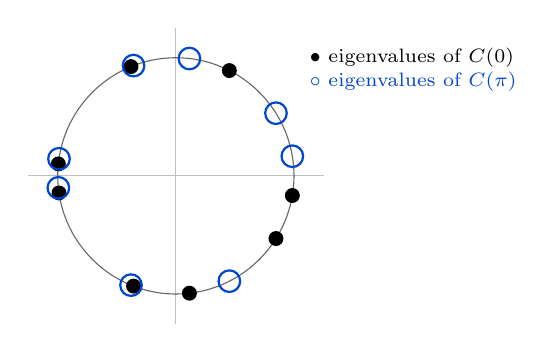
\begin{tikzpicture}[scale=1.5]
\draw[black!25] (-1.25,0)--(1.25,0) (0,-1.25)--(0,1.25);
\draw[black!60] (0,0) circle (1);
\fill[black] (0.4529,0.8916) circle (1.8pt);
\fill[black] (-0.3798,0.9251) circle (1.8pt);
\fill[black] (0.9861,-0.1663) circle (1.8pt);
\fill[black] (0.8475,-0.5307) circle (1.8pt);
\fill[black] (-0.9949,0.1012) circle (1.8pt);
\fill[black] (-0.9895,-0.1445) circle (1.8pt);
\fill[black] (-0.3583,-0.9336) circle (1.8pt);
\fill[black] (0.1148,-0.9934) circle (1.8pt);
\draw[cmid,thick] (0.4529,-0.8916) circle (2.6pt);
\draw[cmid,thick] (-0.3798,-0.9251) circle (2.6pt);
\draw[cmid,thick] (0.9861,0.1663) circle (2.6pt);
\draw[cmid,thick] (0.8475,0.5307) circle (2.6pt);
\draw[cmid,thick] (-0.9949,-0.1012) circle (2.6pt);
\draw[cmid,thick] (-0.9895,0.1445) circle (2.6pt);
\draw[cmid,thick] (-0.3583,0.9336) circle (2.6pt);
\draw[cmid,thick] (0.1148,0.9934) circle (2.6pt);
\node[font=\scriptsize,anchor=west] at (1.05,1.0) {$\bullet$ eigenvalues of $C(0)$};
\node[font=\scriptsize,anchor=west,text=cmid] at (1.05,0.8) {$\circ$ eigenvalues of $C(\pi)$};
\end{tikzpicture}
\caption{Endpoint spectra. The eigenvalues of $C(\pi)$ (blue rings) are the complex conjugates of
those of $C(0)$ (black dots), by $C(\pi)=C(0)^\dagger=C(0)^{-1}$ (Eq.~10).}
\label{fig:endpoints}
\end{figure}

If we list the eigenphases in increasing order, negation reverses the list. The middle half of a
list is unchanged by reversal, and so are the outer quarters. So if we could follow one sorted list
continuously from $\beta=0$ to $\beta=\pi$, the imbalance ``middle half minus outer quarters'' would
start at some value and end at its negative, and would vanish in between. The difficulty is that
eigenphases live on a circle: a sorted list of real numbers needs a choice of $2\pi$ branches, and
that choice must be the same, up to the reversal, at both ends. This is what $\alpha$ is for.

\section*{3. Choosing $\alpha$: making the total phase reverse too}

The branches of a sorted list (span at most $2\pi$) are fixed by its sum, the phase of $\det C$.
For the list at $\beta=\pi$ to be the reversed negative of the list at $\beta=0$, this total
phase $\sigma(\beta)$ must itself go from $\sigma(0)$ to $-\sigma(0)$. Section~II.C shows that
$\sigma$ changes by
\[
\sum_k \operatorname{sgn}(t_k)\,\pi-2\sum_k t_k,\qquad t_k=\arg\tau_k,\quad \tau_k=e^{i\alpha}\rho_k,
\]
where $\rho_k$ are the eigenvalues of $X^{-1}Y$. The unwanted half-turn sum vanishes exactly when
$D/2$ of the $\tau_k$ lie above the real axis and $D/2$ below (Fig.~\ref{fig:alpha}a). Changing
$\alpha$ rotates all $\tau_k$ together, and the upper count $N(\alpha)$ changes only when some
$\tau_k$ crosses the real axis, at $\alpha\equiv-\arg\rho_k\pmod\pi$. So the search for $\alpha$ is a
scan: sort the crossing angles, read off the count on each interval between them, and take the
midpoint of an interval with $N=D/2$ (Fig.~\ref{fig:alpha}b). Such an interval exists because a
half-turn maps $N$ to $D-N$ and $N$ moves in unit steps. With this $\alpha$, $\sigma$ is
antisymmetric on the path (Fig.~\ref{fig:alpha}c).

\begin{figure}[H]
\centering
\begin{minipage}[b]{0.3\textwidth}\centering
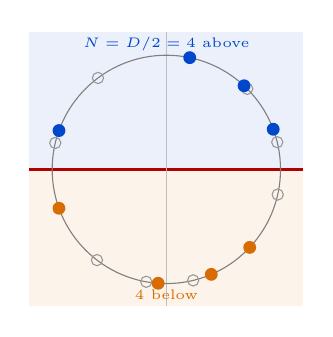
\begin{tikzpicture}[scale=1.45]
\fill[cmid!8] (-1.2,0) rectangle (1.2,1.2);
\fill[cout!8] (-1.2,-1.2) rectangle (1.2,0);
\draw[red!70!black, very thick] (-1.2,0)--(1.2,0);
\draw[black!25] (0,-1.2)--(0,1.2);
\draw[black!50] (0,0) circle (1);
\draw[black!40] (-0.9727,0.2319) circle (1.4pt);
\draw[black!40] (0.2349,-0.9720) circle (1.4pt);
\draw[black!40] (0.9712,0.2384) circle (1.4pt);
\draw[black!40] (0.9755,-0.2201) circle (1.4pt);
\draw[black!40] (0.7087,0.7055) circle (1.4pt);
\draw[black!40] (-0.5988,0.8009) circle (1.4pt);
\draw[black!40] (-0.6077,-0.7942) circle (1.4pt);
\draw[black!40] (-0.1758,-0.9844) circle (1.4pt);
\fill[cout] (-0.9403,-0.3404) circle (1.6pt);
\fill[cout] (0.7302,-0.6833) circle (1.6pt);
\fill[cmid] (0.6807,0.7326) circle (1.6pt);
\fill[cmid] (0.9361,0.3518) circle (1.6pt);
\fill[cmid] (0.2048,0.9788) circle (1.6pt);
\fill[cmid] (-0.9403,0.3404) circle (1.6pt);
\fill[cout] (-0.0717,-0.9974) circle (1.6pt);
\fill[cout] (0.3937,-0.9192) circle (1.6pt);
\node[font=\tiny,text=cmid] at (0,1.1) {$N=D/2=4$ above};
\node[font=\tiny,text=cout] at (0,-1.1) {$4$ below};
\end{tikzpicture}\\[2pt]
{\small (a) directions of $\tau_k$}
\end{minipage}\hfill
\begin{minipage}[b]{0.34\textwidth}\centering
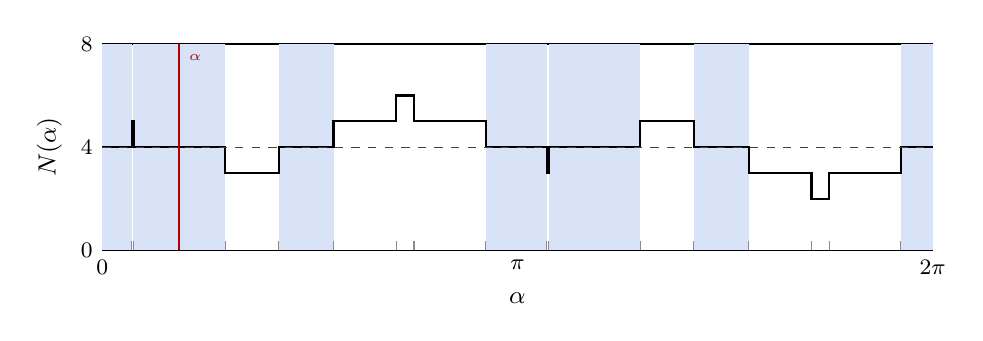
\begin{tikzpicture}
\begin{axis}[width=\linewidth, height=4.2cm, xmin=0, xmax=6.2832, ymin=0, ymax=8,
  xtick={0,3.1416,6.2832}, xticklabels={$0$,$\pi$,$2\pi$}, ytick={0,4,8},
  xlabel={$\alpha$}, ylabel={$N(\alpha)$}, clip=false]
\fill[cmid!15] (axis cs:0.0000,0) rectangle (axis cs:0.2225,8);
\fill[cmid!15] (axis cs:0.2356,0) rectangle (axis cs:0.9294,8);
\fill[cmid!15] (axis cs:1.3352,0) rectangle (axis cs:1.7497,8);
\fill[cmid!15] (axis cs:2.9016,0) rectangle (axis cs:3.3641,8);
\fill[cmid!15] (axis cs:3.3772,0) rectangle (axis cs:4.0710,8);
\fill[cmid!15] (axis cs:4.4768,0) rectangle (axis cs:4.8913,8);
\fill[cmid!15] (axis cs:6.0432,0) rectangle (axis cs:6.2832,8);
\draw[black!45] (axis cs:0.2219,0) -- (axis cs:0.2219,0.35);
\draw[black!45] (axis cs:0.2341,0) -- (axis cs:0.2341,0.35);
\draw[black!45] (axis cs:0.9288,0) -- (axis cs:0.9288,0.35);
\draw[black!45] (axis cs:1.3336,0) -- (axis cs:1.3336,0.35);
\draw[black!45] (axis cs:1.7476,0) -- (axis cs:1.7476,0.35);
\draw[black!45] (axis cs:2.2239,0) -- (axis cs:2.2239,0.35);
\draw[black!45] (axis cs:2.3585,0) -- (axis cs:2.3585,0.35);
\draw[black!45] (axis cs:2.9009,0) -- (axis cs:2.9009,0.35);
\draw[black!45] (axis cs:3.3635,0) -- (axis cs:3.3635,0.35);
\draw[black!45] (axis cs:3.3757,0) -- (axis cs:3.3757,0.35);
\draw[black!45] (axis cs:4.0704,0) -- (axis cs:4.0704,0.35);
\draw[black!45] (axis cs:4.4752,0) -- (axis cs:4.4752,0.35);
\draw[black!45] (axis cs:4.8892,0) -- (axis cs:4.8892,0.35);
\draw[black!45] (axis cs:5.3655,0) -- (axis cs:5.3655,0.35);
\draw[black!45] (axis cs:5.5001,0) -- (axis cs:5.5001,0.35);
\draw[black!45] (axis cs:6.0425,0) -- (axis cs:6.0425,0.35);
\addplot[black, thick, const plot] coordinates {(0.0000,4) (0.2225,5) (0.2356,4) (0.9294,3) (1.3352,4) (1.7497,5) (2.2253,6) (2.3606,5) (2.9016,4) (3.3641,3) (3.3772,4) (4.0710,5) (4.4768,4) (4.8913,3) (5.3669,2) (5.5022,3) (6.0432,4) (6.2832,4)};
\addplot[cmid, dashed] coordinates {(0,4) (6.2832,4)};
\draw[red!70!black, thick] (axis cs:0.5814,0) -- (axis cs:0.5814,8);
\node[font=\tiny, text=red!70!black, anchor=south west] at (axis cs:0.5814,7) {$\alpha$};
\end{axis}
\end{tikzpicture}\\[2pt]
{\small (b) upper-half-plane count}
\end{minipage}\hfill
\begin{minipage}[b]{0.34\textwidth}\centering
\begin{tikzpicture}
\begin{axis}[width=\linewidth, height=4.2cm, xmin=0, xmax=3.1416, xtick={0,1.5708,3.1416},
  xticklabels={$0$,$\pi/2$,$\pi$}, xlabel={$\beta$}, ylabel={$\sigma(\beta)$}]
\addplot[black!30, dotted] coordinates {(0,0) (3.1416,0)};
\addplot[black, thick] coordinates {(0.0000,-1.0147) (0.0262,-0.9883) (0.0524,-0.9620) (0.0785,-0.9355) (0.1047,-0.9089) (0.1309,-0.8821) (0.1571,-0.8549) (0.1833,-0.8274) (0.2094,-0.7993) (0.2356,-0.7707) (0.2618,-0.7413) (0.2880,-0.7112) (0.3142,-0.6801) (0.3403,-0.6479) (0.3665,-0.6144) (0.3927,-0.5795) (0.4189,-0.5429) (0.4451,-0.5045) (0.4712,-0.4639) (0.4974,-0.4208) (0.5236,-0.3749) (0.5498,-0.3258) (0.5760,-0.2732) (0.6021,-0.2164) (0.6283,-0.1552) (0.6545,-0.0890) (0.6807,-0.0173) (0.7069,0.0602) (0.7330,0.1438) (0.7592,0.2335) (0.7854,0.3291) (0.8116,0.4302) (0.8378,0.5356) (0.8639,0.6443) (0.8901,0.7548) (0.9163,0.8654) (0.9425,0.9746) (0.9687,1.0812) (0.9948,1.1842) (1.0210,1.2833) (1.0472,1.3781) (1.0734,1.4688) (1.0996,1.5557) (1.1257,1.6394) (1.1519,1.7203) (1.1781,1.7992) (1.2043,1.8766) (1.2305,1.9531) (1.2566,2.0292) (1.2828,2.1053) (1.3090,2.1819) (1.3352,2.2591) (1.3614,2.3370) (1.3875,2.4158) (1.4137,2.4951) (1.4399,2.5748) (1.4661,2.6543) (1.4923,2.7331) (1.5184,2.8105) (1.5446,2.8860) (1.5708,2.9587) (1.5970,3.0281) (1.6232,3.0937) (1.6493,3.1550) (1.6755,3.2117) (1.7017,3.2635) (1.7279,3.3102) (1.7541,3.3518) (1.7802,3.3883) (1.8064,3.4196) (1.8326,3.4457) (1.8588,3.4667) (1.8850,3.4825) (1.9111,3.4931) (1.9373,3.4985) (1.9635,3.4986) (1.9897,3.4932) (2.0159,3.4823) (2.0420,3.4655) (2.0682,3.4427) (2.0944,3.4134) (2.1206,3.3773) (2.1468,3.3340) (2.1729,3.2829) (2.1991,3.2238) (2.2253,3.1561) (2.2515,3.0797) (2.2777,2.9947) (2.3038,2.9014) (2.3300,2.8010) (2.3562,2.6949) (2.3824,2.5853) (2.4086,2.4745) (2.4347,2.3651) (2.4609,2.2591) (2.4871,2.1583) (2.5133,2.0638) (2.5395,1.9761) (2.5656,1.8954) (2.5918,1.8213) (2.6180,1.7535) (2.6442,1.6913) (2.6704,1.6342) (2.6965,1.5816) (2.7227,1.5330) (2.7489,1.4879) (2.7751,1.4457) (2.8013,1.4062) (2.8274,1.3689) (2.8536,1.3336) (2.8798,1.3000) (2.9060,1.2678) (2.9322,1.2369) (2.9583,1.2070) (2.9845,1.1779) (3.0107,1.1496) (3.0369,1.1219) (3.0631,1.0946) (3.0892,1.0677) (3.1154,1.0411) (3.1416,1.0147)};
\end{axis}
\end{tikzpicture}\\[2pt]
{\small (c) total phase}
\end{minipage}
\caption{Choosing $\alpha$. (a)~At the chosen $\alpha$, half of the directions $\tau_k/|\tau_k|$ lie
above the real axis (blue) and half below (orange); grey rings show $\rho_k$ before rotation, and
no $\tau_k$ may sit on the red axis. (b)~The count $N(\alpha)$ is a step function that jumps at
the crossing angles (ticks); shaded intervals have $N=D/2$, and the code takes the midpoint of the
widest one. (c)~With this $\alpha$, the continuous phase of $\det C$ satisfies
$\sigma(\pi)=-\sigma(0)$ (Eq.~12).}
\label{fig:alpha}
\end{figure}

\section*{4. Choosing $\beta$: bisecting the imbalance}

With $\alpha$ fixed, list the eigenphases of $C(\beta)$ as real numbers
$\nu_0\le\dots\le\nu_{D-1}\le\nu_0+2\pi$ with $\sum_j\nu_j=\sigma(\beta)$. These lifts vary
continuously (Fig.~\ref{fig:beta}a), and at the ends the list is reversed and negated,
$\nu_j(\pi)=-\nu_{D-1-j}(0)$ (Fig.~\ref{fig:beta}b). The middle half $S=\{2,3,4,5\}$ maps to itself
under $j\mapsto D-1-j$, so the imbalance
\[
P(\beta)=\sum_{j\in S}\nu_j(\beta)-\sum_{j\notin S}\nu_j(\beta)
\]
satisfies $P(\pi)=-P(0)$ and has a root, which bisection finds (Fig.~\ref{fig:beta}c). Here
$P(0)=-1.148$, $P(\pi)=1.148$, and $\beta^\ast=1.3950$.

\begin{figure}[H]
\centering
\begin{minipage}[b]{0.48\textwidth}\centering
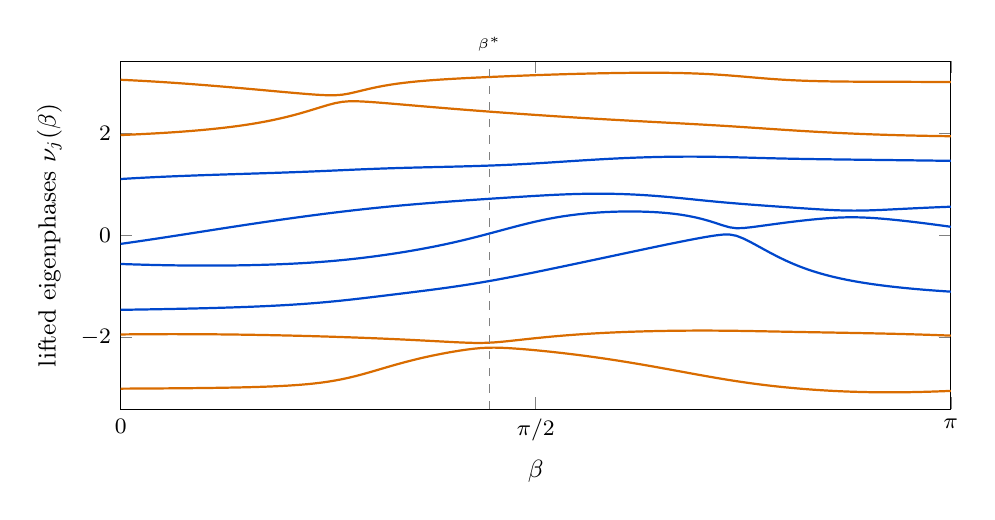
\begin{tikzpicture}
\begin{axis}[width=\linewidth, height=6cm, xmin=0, xmax=3.1416, xtick={0,1.5708,3.1416},
  xticklabels={$0$,$\pi/2$,$\pi$}, xlabel={$\beta$}, ylabel={lifted eigenphases $\nu_j(\beta)$},
  ymin=-3.4, ymax=3.4, clip=false]
\addplot[cout, thick] coordinates {(0.0000,-2.9966) (0.0262,-2.9959) (0.0524,-2.9952) (0.0785,-2.9944) (0.1047,-2.9936) (0.1309,-2.9927) (0.1571,-2.9917) (0.1833,-2.9907) (0.2094,-2.9896) (0.2356,-2.9885) (0.2618,-2.9872) (0.2880,-2.9858) (0.3142,-2.9842) (0.3403,-2.9825) (0.3665,-2.9805) (0.3927,-2.9783) (0.4189,-2.9759) (0.4451,-2.9731) (0.4712,-2.9700) (0.4974,-2.9664) (0.5236,-2.9623) (0.5498,-2.9576) (0.5760,-2.9522) (0.6021,-2.9460) (0.6283,-2.9387) (0.6545,-2.9302) (0.6807,-2.9203) (0.7069,-2.9086) (0.7330,-2.8949) (0.7592,-2.8787) (0.7854,-2.8597) (0.8116,-2.8374) (0.8378,-2.8117) (0.8639,-2.7824) (0.8901,-2.7497) (0.9163,-2.7139) (0.9425,-2.6759) (0.9687,-2.6365) (0.9948,-2.5966) (1.0210,-2.5572) (1.0472,-2.5187) (1.0734,-2.4818) (1.0996,-2.4467) (1.1257,-2.4134) (1.1519,-2.3821) (1.1781,-2.3527) (1.2043,-2.3251) (1.2305,-2.2994) (1.2566,-2.2754) (1.2828,-2.2533) (1.3090,-2.2335) (1.3352,-2.2166) (1.3614,-2.2038) (1.3875,-2.1963) (1.4137,-2.1945) (1.4399,-2.1975) (1.4661,-2.2039) (1.4923,-2.2125) (1.5184,-2.2226) (1.5446,-2.2340) (1.5708,-2.2462) (1.5970,-2.2593) (1.6232,-2.2732) (1.6493,-2.2878) (1.6755,-2.3032) (1.7017,-2.3192) (1.7279,-2.3359) (1.7541,-2.3534) (1.7802,-2.3716) (1.8064,-2.3904) (1.8326,-2.4100) (1.8588,-2.4302) (1.8850,-2.4512) (1.9111,-2.4727) (1.9373,-2.4949) (1.9635,-2.5177) (1.9897,-2.5410) (2.0159,-2.5647) (2.0420,-2.5889) (2.0682,-2.6133) (2.0944,-2.6380) (2.1206,-2.6628) (2.1468,-2.6876) (2.1729,-2.7123) (2.1991,-2.7367) (2.2253,-2.7607) (2.2515,-2.7842) (2.2777,-2.8070) (2.3038,-2.8290) (2.3300,-2.8501) (2.3562,-2.8703) (2.3824,-2.8893) (2.4086,-2.9074) (2.4347,-2.9244) (2.4609,-2.9404) (2.4871,-2.9553) (2.5133,-2.9693) (2.5395,-2.9823) (2.5656,-2.9943) (2.5918,-3.0054) (2.6180,-3.0156) (2.6442,-3.0249) (2.6704,-3.0332) (2.6965,-3.0407) (2.7227,-3.0472) (2.7489,-3.0529) (2.7751,-3.0576) (2.8013,-3.0615) (2.8274,-3.0645) (2.8536,-3.0667) (2.8798,-3.0680) (2.9060,-3.0685) (2.9322,-3.0681) (2.9583,-3.0670) (2.9845,-3.0652) (3.0107,-3.0627) (3.0369,-3.0594) (3.0631,-3.0555) (3.0892,-3.0510) (3.1154,-3.0459) (3.1416,-3.0403)};
\addplot[cout, thick] coordinates {(0.0000,-1.9372) (0.0262,-1.9356) (0.0524,-1.9343) (0.0785,-1.9332) (0.1047,-1.9324) (0.1309,-1.9317) (0.1571,-1.9313) (0.1833,-1.9311) (0.2094,-1.9311) (0.2356,-1.9313) (0.2618,-1.9317) (0.2880,-1.9323) (0.3142,-1.9332) (0.3403,-1.9342) (0.3665,-1.9354) (0.3927,-1.9367) (0.4189,-1.9383) (0.4451,-1.9401) (0.4712,-1.9420) (0.4974,-1.9442) (0.5236,-1.9465) (0.5498,-1.9490) (0.5760,-1.9516) (0.6021,-1.9545) (0.6283,-1.9575) (0.6545,-1.9607) (0.6807,-1.9641) (0.7069,-1.9677) (0.7330,-1.9714) (0.7592,-1.9753) (0.7854,-1.9794) (0.8116,-1.9837) (0.8378,-1.9881) (0.8639,-1.9928) (0.8901,-1.9976) (0.9163,-2.0027) (0.9425,-2.0079) (0.9687,-2.0134) (0.9948,-2.0190) (1.0210,-2.0250) (1.0472,-2.0311) (1.0734,-2.0374) (1.0996,-2.0440) (1.1257,-2.0508) (1.1519,-2.0577) (1.1781,-2.0648) (1.2043,-2.0720) (1.2305,-2.0791) (1.2566,-2.0861) (1.2828,-2.0926) (1.3090,-2.0982) (1.3352,-2.1022) (1.3614,-2.1033) (1.3875,-2.1002) (1.4137,-2.0925) (1.4399,-2.0813) (1.4661,-2.0678) (1.4923,-2.0532) (1.5184,-2.0384) (1.5446,-2.0237) (1.5708,-2.0095) (1.5970,-1.9958) (1.6232,-1.9828) (1.6493,-1.9706) (1.6755,-1.9591) (1.7017,-1.9484) (1.7279,-1.9384) (1.7541,-1.9293) (1.7802,-1.9208) (1.8064,-1.9130) (1.8326,-1.9059) (1.8588,-1.8994) (1.8850,-1.8935) (1.9111,-1.8882) (1.9373,-1.8835) (1.9635,-1.8792) (1.9897,-1.8755) (2.0159,-1.8722) (2.0420,-1.8693) (2.0682,-1.8670) (2.0944,-1.8650) (2.1206,-1.8635) (2.1468,-1.8624) (2.1729,-1.8618) (2.1991,-1.8615) (2.2253,-1.8617) (2.2515,-1.8623) (2.2777,-1.8633) (2.3038,-1.8647) (2.3300,-1.8664) (2.3562,-1.8684) (2.3824,-1.8707) (2.4086,-1.8731) (2.4347,-1.8757) (2.4609,-1.8784) (2.4871,-1.8810) (2.5133,-1.8836) (2.5395,-1.8862) (2.5656,-1.8887) (2.5918,-1.8912) (2.6180,-1.8936) (2.6442,-1.8960) (2.6704,-1.8984) (2.6965,-1.9007) (2.7227,-1.9031) (2.7489,-1.9056) (2.7751,-1.9081) (2.8013,-1.9107) (2.8274,-1.9134) (2.8536,-1.9162) (2.8798,-1.9192) (2.9060,-1.9223) (2.9322,-1.9256) (2.9583,-1.9291) (2.9845,-1.9328) (3.0107,-1.9367) (3.0369,-1.9409) (3.0631,-1.9453) (3.0892,-1.9500) (3.1154,-1.9550) (3.1416,-1.9603)};
\addplot[cmid, thick] coordinates {(0.0000,-1.4558) (0.0262,-1.4538) (0.0524,-1.4517) (0.0785,-1.4495) (0.1047,-1.4473) (0.1309,-1.4449) (0.1571,-1.4425) (0.1833,-1.4399) (0.2094,-1.4372) (0.2356,-1.4344) (0.2618,-1.4314) (0.2880,-1.4282) (0.3142,-1.4249) (0.3403,-1.4214) (0.3665,-1.4176) (0.3927,-1.4136) (0.4189,-1.4094) (0.4451,-1.4048) (0.4712,-1.4000) (0.4974,-1.3948) (0.5236,-1.3891) (0.5498,-1.3831) (0.5760,-1.3766) (0.6021,-1.3695) (0.6283,-1.3619) (0.6545,-1.3536) (0.6807,-1.3447) (0.7069,-1.3350) (0.7330,-1.3245) (0.7592,-1.3132) (0.7854,-1.3010) (0.8116,-1.2880) (0.8378,-1.2742) (0.8639,-1.2597) (0.8901,-1.2446) (0.9163,-1.2290) (0.9425,-1.2130) (0.9687,-1.1968) (0.9948,-1.1805) (1.0210,-1.1640) (1.0472,-1.1475) (1.0734,-1.1310) (1.0996,-1.1143) (1.1257,-1.0975) (1.1519,-1.0803) (1.1781,-1.0629) (1.2043,-1.0450) (1.2305,-1.0265) (1.2566,-1.0074) (1.2828,-0.9876) (1.3090,-0.9670) (1.3352,-0.9456) (1.3614,-0.9232) (1.3875,-0.9001) (1.4137,-0.8760) (1.4399,-0.8512) (1.4661,-0.8257) (1.4923,-0.7995) (1.5184,-0.7727) (1.5446,-0.7456) (1.5708,-0.7181) (1.5970,-0.6903) (1.6232,-0.6623) (1.6493,-0.6341) (1.6755,-0.6058) (1.7017,-0.5774) (1.7279,-0.5490) (1.7541,-0.5204) (1.7802,-0.4918) (1.8064,-0.4631) (1.8326,-0.4344) (1.8588,-0.4056) (1.8850,-0.3769) (1.9111,-0.3481) (1.9373,-0.3193) (1.9635,-0.2906) (1.9897,-0.2620) (2.0159,-0.2336) (2.0420,-0.2054) (2.0682,-0.1775) (2.0944,-0.1499) (2.1206,-0.1227) (2.1468,-0.0961) (2.1729,-0.0703) (2.1991,-0.0454) (2.2253,-0.0221) (2.2515,-0.0013) (2.2777,0.0142) (2.3038,0.0166) (2.3300,-0.0085) (2.3562,-0.0614) (2.3824,-0.1285) (2.4086,-0.2013) (2.4347,-0.2756) (2.4609,-0.3487) (2.4871,-0.4186) (2.5133,-0.4844) (2.5395,-0.5452) (2.5656,-0.6009) (2.5918,-0.6517) (2.6180,-0.6977) (2.6442,-0.7393) (2.6704,-0.7770) (2.6965,-0.8111) (2.7227,-0.8420) (2.7489,-0.8701) (2.7751,-0.8957) (2.8013,-0.9191) (2.8274,-0.9405) (2.8536,-0.9601) (2.8798,-0.9782) (2.9060,-0.9949) (2.9322,-1.0103) (2.9583,-1.0246) (2.9845,-1.0379) (3.0107,-1.0502) (3.0369,-1.0617) (3.0631,-1.0725) (3.0892,-1.0825) (3.1154,-1.0920) (3.1416,-1.1008)};
\addplot[cmid, thick] coordinates {(0.0000,-0.5595) (0.0262,-0.5642) (0.0524,-0.5687) (0.0785,-0.5727) (0.1047,-0.5764) (0.1309,-0.5796) (0.1571,-0.5825) (0.1833,-0.5850) (0.2094,-0.5871) (0.2356,-0.5887) (0.2618,-0.5900) (0.2880,-0.5909) (0.3142,-0.5913) (0.3403,-0.5913) (0.3665,-0.5909) (0.3927,-0.5900) (0.4189,-0.5887) (0.4451,-0.5869) (0.4712,-0.5846) (0.4974,-0.5818) (0.5236,-0.5784) (0.5498,-0.5745) (0.5760,-0.5700) (0.6021,-0.5649) (0.6283,-0.5592) (0.6545,-0.5527) (0.6807,-0.5455) (0.7069,-0.5375) (0.7330,-0.5287) (0.7592,-0.5189) (0.7854,-0.5083) (0.8116,-0.4966) (0.8378,-0.4839) (0.8639,-0.4702) (0.8901,-0.4555) (0.9163,-0.4398) (0.9425,-0.4230) (0.9687,-0.4053) (0.9948,-0.3866) (1.0210,-0.3669) (1.0472,-0.3463) (1.0734,-0.3247) (1.0996,-0.3021) (1.1257,-0.2784) (1.1519,-0.2536) (1.1781,-0.2277) (1.2043,-0.2005) (1.2305,-0.1721) (1.2566,-0.1424) (1.2828,-0.1114) (1.3090,-0.0790) (1.3352,-0.0455) (1.3614,-0.0109) (1.3875,0.0246) (1.4137,0.0607) (1.4399,0.0972) (1.4661,0.1336) (1.4923,0.1694) (1.5184,0.2044) (1.5446,0.2379) (1.5708,0.2696) (1.5970,0.2991) (1.6232,0.3263) (1.6493,0.3509) (1.6755,0.3729) (1.7017,0.3924) (1.7279,0.4093) (1.7541,0.4238) (1.7802,0.4360) (1.8064,0.4461) (1.8326,0.4540) (1.8588,0.4600) (1.8850,0.4641) (1.9111,0.4663) (1.9373,0.4665) (1.9635,0.4649) (1.9897,0.4611) (2.0159,0.4551) (2.0420,0.4467) (2.0682,0.4354) (2.0944,0.4210) (2.1206,0.4028) (2.1468,0.3805) (2.1729,0.3534) (2.1991,0.3211) (2.2253,0.2835) (2.2515,0.2411) (2.2777,0.1964) (2.3038,0.1574) (2.3300,0.1390) (2.3562,0.1427) (2.3824,0.1565) (2.4086,0.1738) (2.4347,0.1922) (2.4609,0.2107) (2.4871,0.2289) (2.5133,0.2467) (2.5395,0.2637) (2.5656,0.2798) (2.5918,0.2950) (2.6180,0.3090) (2.6442,0.3217) (2.6704,0.3328) (2.6965,0.3419) (2.7227,0.3486) (2.7489,0.3524) (2.7751,0.3530) (2.8013,0.3503) (2.8274,0.3446) (2.8536,0.3364) (2.8798,0.3261) (2.9060,0.3142) (2.9322,0.3010) (2.9583,0.2867) (2.9845,0.2715) (3.0107,0.2555) (3.0369,0.2389) (3.0631,0.2217) (3.0892,0.2040) (3.1154,0.1857) (3.1416,0.1671)};
\addplot[cmid, thick] coordinates {(0.0000,-0.1671) (0.0262,-0.1480) (0.0524,-0.1285) (0.0785,-0.1088) (0.1047,-0.0887) (0.1309,-0.0684) (0.1571,-0.0479) (0.1833,-0.0272) (0.2094,-0.0063) (0.2356,0.0146) (0.2618,0.0357) (0.2880,0.0568) (0.3142,0.0779) (0.3403,0.0990) (0.3665,0.1201) (0.3927,0.1410) (0.4189,0.1619) (0.4451,0.1826) (0.4712,0.2032) (0.4974,0.2235) (0.5236,0.2437) (0.5498,0.2636) (0.5760,0.2833) (0.6021,0.3027) (0.6283,0.3218) (0.6545,0.3406) (0.6807,0.3591) (0.7069,0.3773) (0.7330,0.3952) (0.7592,0.4127) (0.7854,0.4298) (0.8116,0.4465) (0.8378,0.4629) (0.8639,0.4788) (0.8901,0.4943) (0.9163,0.5093) (0.9425,0.5239) (0.9687,0.5380) (0.9948,0.5516) (1.0210,0.5647) (1.0472,0.5774) (1.0734,0.5897) (1.0996,0.6016) (1.1257,0.6130) (1.1519,0.6241) (1.1781,0.6348) (1.2043,0.6452) (1.2305,0.6554) (1.2566,0.6652) (1.2828,0.6748) (1.3090,0.6843) (1.3352,0.6935) (1.3614,0.7026) (1.3875,0.7116) (1.4137,0.7206) (1.4399,0.7294) (1.4661,0.7381) (1.4923,0.7468) (1.5184,0.7553) (1.5446,0.7637) (1.5708,0.7718) (1.5970,0.7795) (1.6232,0.7868) (1.6493,0.7934) (1.6755,0.7994) (1.7017,0.8045) (1.7279,0.8086) (1.7541,0.8117) (1.7802,0.8136) (1.8064,0.8143) (1.8326,0.8138) (1.8588,0.8119) (1.8850,0.8088) (1.9111,0.8044) (1.9373,0.7987) (1.9635,0.7916) (1.9897,0.7834) (2.0159,0.7739) (2.0420,0.7633) (2.0682,0.7517) (2.0944,0.7393) (2.1206,0.7262) (2.1468,0.7127) (2.1729,0.6990) (2.1991,0.6853) (2.2253,0.6719) (2.2515,0.6589) (2.2777,0.6465) (2.3038,0.6345) (2.3300,0.6232) (2.3562,0.6122) (2.3824,0.6017) (2.4086,0.5916) (2.4347,0.5817) (2.4609,0.5720) (2.4871,0.5624) (2.5133,0.5529) (2.5395,0.5435) (2.5656,0.5342) (2.5918,0.5251) (2.6180,0.5162) (2.6442,0.5078) (2.6704,0.5000) (2.6965,0.4932) (2.7227,0.4879) (2.7489,0.4844) (2.7751,0.4831) (2.8013,0.4841) (2.8274,0.4871) (2.8536,0.4917) (2.8798,0.4973) (2.9060,0.5036) (2.9322,0.5103) (2.9583,0.5171) (2.9845,0.5238) (3.0107,0.5304) (3.0369,0.5368) (3.0631,0.5430) (3.0892,0.5488) (3.1154,0.5543) (3.1416,0.5595)};
\addplot[cmid, thick] coordinates {(0.0000,1.1008) (0.0262,1.1091) (0.0524,1.1170) (0.0785,1.1244) (0.1047,1.1314) (0.1309,1.1380) (0.1571,1.1442) (0.1833,1.1502) (0.2094,1.1558) (0.2356,1.1612) (0.2618,1.1664) (0.2880,1.1714) (0.3142,1.1762) (0.3403,1.1808) (0.3665,1.1853) (0.3927,1.1897) (0.4189,1.1940) (0.4451,1.1983) (0.4712,1.2025) (0.4974,1.2068) (0.5236,1.2111) (0.5498,1.2154) (0.5760,1.2199) (0.6021,1.2244) (0.6283,1.2292) (0.6545,1.2341) (0.6807,1.2392) (0.7069,1.2445) (0.7330,1.2500) (0.7592,1.2557) (0.7854,1.2615) (0.8116,1.2675) (0.8378,1.2735) (0.8639,1.2795) (0.8901,1.2853) (0.9163,1.2910) (0.9425,1.2964) (0.9687,1.3015) (0.9948,1.3064) (1.0210,1.3109) (1.0472,1.3151) (1.0734,1.3190) (1.0996,1.3227) (1.1257,1.3262) (1.1519,1.3295) (1.1781,1.3328) (1.2043,1.3360) (1.2305,1.3392) (1.2566,1.3425) (1.2828,1.3459) (1.3090,1.3495) (1.3352,1.3534) (1.3614,1.3575) (1.3875,1.3621) (1.4137,1.3670) (1.4399,1.3724) (1.4661,1.3783) (1.4923,1.3847) (1.5184,1.3916) (1.5446,1.3989) (1.5708,1.4067) (1.5970,1.4149) (1.6232,1.4234) (1.6493,1.4321) (1.6755,1.4409) (1.7017,1.4497) (1.7279,1.4585) (1.7541,1.4670) (1.7802,1.4753) (1.8064,1.4833) (1.8326,1.4909) (1.8588,1.4981) (1.8850,1.5047) (1.9111,1.5108) (1.9373,1.5164) (1.9635,1.5214) (1.9897,1.5257) (2.0159,1.5295) (2.0420,1.5326) (2.0682,1.5351) (2.0944,1.5369) (2.1206,1.5380) (2.1468,1.5385) (2.1729,1.5384) (2.1991,1.5376) (2.2253,1.5361) (2.2515,1.5341) (2.2777,1.5315) (2.3038,1.5285) (2.3300,1.5251) (2.3562,1.5214) (2.3824,1.5177) (2.4086,1.5139) (2.4347,1.5102) (2.4609,1.5067) (2.4871,1.5034) (2.5133,1.5004) (2.5395,1.4976) (2.5656,1.4950) (2.5918,1.4926) (2.6180,1.4904) (2.6442,1.4884) (2.6704,1.4864) (2.6965,1.4846) (2.7227,1.4828) (2.7489,1.4811) (2.7751,1.4795) (2.8013,1.4779) (2.8274,1.4763) (2.8536,1.4747) (2.8798,1.4731) (2.9060,1.4715) (2.9322,1.4699) (2.9583,1.4683) (2.9845,1.4666) (3.0107,1.4649) (3.0369,1.4632) (3.0631,1.4614) (3.0892,1.4596) (3.1154,1.4577) (3.1416,1.4558)};
\addplot[cout, thick] coordinates {(0.0000,1.9603) (0.0262,1.9660) (0.0524,1.9721) (0.0785,1.9785) (0.1047,1.9854) (0.1309,1.9928) (0.1571,2.0007) (0.1833,2.0092) (0.2094,2.0182) (0.2356,2.0279) (0.2618,2.0384) (0.2880,2.0496) (0.3142,2.0617) (0.3403,2.0747) (0.3665,2.0887) (0.3927,2.1039) (0.4189,2.1203) (0.4451,2.1382) (0.4712,2.1575) (0.4974,2.1785) (0.5236,2.2014) (0.5498,2.2263) (0.5760,2.2533) (0.6021,2.2828) (0.6283,2.3147) (0.6545,2.3492) (0.6807,2.3862) (0.7069,2.4255) (0.7330,2.4665) (0.7592,2.5082) (0.7854,2.5486) (0.8116,2.5839) (0.8378,2.6088) (0.8639,2.6202) (0.8901,2.6210) (0.9163,2.6158) (0.9425,2.6076) (0.9687,2.5978) (0.9948,2.5871) (1.0210,2.5760) (1.0472,2.5646) (1.0734,2.5530) (1.0996,2.5415) (1.1257,2.5300) (1.1519,2.5185) (1.1781,2.5071) (1.2043,2.4959) (1.2305,2.4848) (1.2566,2.4738) (1.2828,2.4629) (1.3090,2.4523) (1.3352,2.4417) (1.3614,2.4313) (1.3875,2.4211) (1.4137,2.4110) (1.4399,2.4011) (1.4661,2.3913) (1.4923,2.3816) (1.5184,2.3720) (1.5446,2.3626) (1.5708,2.3534) (1.5970,2.3443) (1.6232,2.3353) (1.6493,2.3264) (1.6755,2.3177) (1.7017,2.3092) (1.7279,2.3007) (1.7541,2.2925) (1.7802,2.2843) (1.8064,2.2763) (1.8326,2.2685) (1.8588,2.2607) (1.8850,2.2531) (1.9111,2.2456) (1.9373,2.2381) (1.9635,2.2308) (1.9897,2.2235) (2.0159,2.2163) (2.0420,2.2091) (2.0682,2.2019) (2.0944,2.1948) (2.1206,2.1875) (2.1468,2.1802) (2.1729,2.1728) (2.1991,2.1653) (2.2253,2.1576) (2.2515,2.1497) (2.2777,2.1416) (2.3038,2.1333) (2.3300,2.1247) (2.3562,2.1158) (2.3824,2.1069) (2.4086,2.0977) (2.4347,2.0886) (2.4609,2.0794) (2.4871,2.0703) (2.5133,2.0614) (2.5395,2.0527) (2.5656,2.0442) (2.5918,2.0360) (2.6180,2.0281) (2.6442,2.0205) (2.6704,2.0133) (2.6965,2.0063) (2.7227,1.9998) (2.7489,1.9935) (2.7751,1.9876) (2.8013,1.9820) (2.8274,1.9768) (2.8536,1.9719) (2.8798,1.9673) (2.9060,1.9630) (2.9322,1.9590) (2.9583,1.9553) (2.9845,1.9519) (3.0107,1.9488) (3.0369,1.9459) (3.0631,1.9434) (3.0892,1.9410) (3.1154,1.9390) (3.1416,1.9372)};
\addplot[cout, thick] coordinates {(0.0000,3.0403) (0.0262,3.0341) (0.0524,3.0274) (0.0785,3.0202) (0.1047,3.0126) (0.1309,3.0045) (0.1571,2.9961) (0.1833,2.9872) (0.2094,2.9780) (0.2356,2.9684) (0.2618,2.9585) (0.2880,2.9483) (0.3142,2.9378) (0.3403,2.9270) (0.3665,2.9159) (0.3927,2.9046) (0.4189,2.8931) (0.4451,2.8814) (0.4712,2.8695) (0.4974,2.8575) (0.5236,2.8453) (0.5498,2.8331) (0.5760,2.8208) (0.6021,2.8086) (0.6283,2.7964) (0.6545,2.7845) (0.6807,2.7728) (0.7069,2.7617) (0.7330,2.7515) (0.7592,2.7430) (0.7854,2.7376) (0.8116,2.7380) (0.8378,2.7485) (0.8639,2.7710) (0.8901,2.8016) (0.9163,2.8346) (0.9425,2.8665) (0.9687,2.8958) (0.9948,2.9219) (1.0210,2.9448) (1.0472,2.9646) (1.0734,2.9819) (1.0996,2.9970) (1.1257,3.0103) (1.1519,3.0221) (1.1781,3.0327) (1.2043,3.0422) (1.2305,3.0509) (1.2566,3.0590) (1.2828,3.0665) (1.3090,3.0736) (1.3352,3.0804) (1.3614,3.0868) (1.3875,3.0930) (1.4137,3.0989) (1.4399,3.1047) (1.4661,3.1103) (1.4923,3.1158) (1.5184,3.1210) (1.5446,3.1261) (1.5708,3.1310) (1.5970,3.1358) (1.6232,3.1403) (1.6493,3.1447) (1.6755,3.1488) (1.7017,3.1527) (1.7279,3.1564) (1.7541,3.1599) (1.7802,3.1631) (1.8064,3.1661) (1.8326,3.1688) (1.8588,3.1712) (1.8850,3.1733) (1.9111,3.1751) (1.9373,3.1764) (1.9635,3.1774) (1.9897,3.1779) (2.0159,3.1780) (2.0420,3.1774) (2.0682,3.1763) (2.0944,3.1744) (2.1206,3.1718) (2.1468,3.1682) (2.1729,3.1637) (2.1991,3.1582) (2.2253,3.1516) (2.2515,3.1438) (2.2777,3.1349) (2.3038,3.1249) (2.3300,3.1141) (2.3562,3.1027) (2.3824,3.0910) (2.4086,3.0794) (2.4347,3.0682) (2.4609,3.0577) (2.4871,3.0482) (2.5133,3.0397) (2.5395,3.0324) (2.5656,3.0261) (2.5918,3.0209) (2.6180,3.0166) (2.6442,3.0131) (2.6704,3.0103) (2.6965,3.0080) (2.7227,3.0063) (2.7489,3.0050) (2.7751,3.0039) (2.8013,3.0032) (2.8274,3.0025) (2.8536,3.0020) (2.8798,3.0016) (2.9060,3.0012) (2.9322,3.0008) (2.9583,3.0004) (2.9845,3.0000) (3.0107,2.9995) (3.0369,2.9990) (3.0631,2.9985) (3.0892,2.9979) (3.1154,2.9973) (3.1416,2.9966)};
\draw[black!50, dashed] (axis cs:1.3950,-3.4) -- (axis cs:1.3950,3.4);
\node[font=\tiny, anchor=south] at (axis cs:1.3950,3.4) {$\beta^\ast$};
\end{axis}
\end{tikzpicture}\\[2pt]
{\small (a) the sorted, lifted list along the path}
\end{minipage}\hfill
\begin{minipage}[b]{0.48\textwidth}\centering
\begin{tikzpicture}
\begin{axis}[width=\linewidth, height=6cm, xmin=0, xmax=3.1416, xtick={0,1.5708,3.1416},
  xticklabels={$0$,$\pi/2$,$\pi$}, xlabel={$\beta$}, ylabel={imbalance $P(\beta)$}, clip=false]
\addplot[black!30, dotted] coordinates {(0,0) (3.1416,0)};
\addplot[black, thick] coordinates {(0.0000,-1.1483) (0.0262,-1.1254) (0.0524,-1.1019) (0.0785,-1.0778) (0.1047,-1.0531) (0.1309,-1.0280) (0.1571,-1.0024) (0.1833,-0.9765) (0.2094,-0.9503) (0.2356,-0.9238) (0.2618,-0.8973) (0.2880,-0.8707) (0.3142,-0.8442) (0.3403,-0.8179) (0.3665,-0.7919) (0.3927,-0.7663) (0.4189,-0.7414) (0.4451,-0.7171) (0.4712,-0.6938) (0.4974,-0.6716) (0.5236,-0.6507) (0.5498,-0.6314) (0.5760,-0.6138) (0.6021,-0.5983) (0.6283,-0.5851) (0.6545,-0.5744) (0.6807,-0.5665) (0.7069,-0.5616) (0.7330,-0.5598) (0.7592,-0.5610) (0.7854,-0.5650) (0.8116,-0.5713) (0.8378,-0.5792) (0.8639,-0.5877) (0.8901,-0.5958) (0.9163,-0.6023) (0.9425,-0.6061) (0.9687,-0.6064) (0.9948,-0.6025) (1.0210,-0.5940) (1.0472,-0.5807) (1.0734,-0.5627) (1.0996,-0.5400) (1.1257,-0.5128) (1.1519,-0.4811) (1.1781,-0.4452) (1.2043,-0.4053) (1.2305,-0.3613) (1.2566,-0.3135) (1.2828,-0.2618) (1.3090,-0.2065) (1.3352,-0.1475) (1.3614,-0.0851) (1.3875,-0.0194) (1.4137,0.0494) (1.4399,0.1207) (1.4661,0.1944) (1.4923,0.2698) (1.5184,0.3465) (1.5446,0.4238) (1.5708,0.5013) (1.5970,0.5784) (1.6232,0.6546) (1.6493,0.7296) (1.6755,0.8031) (1.7017,0.8748) (1.7279,0.9446) (1.7541,1.0124) (1.7802,1.0780) (1.8064,1.1416) (1.8326,1.2029) (1.8588,1.2621) (1.8850,1.3191) (1.9111,1.3737) (1.9373,1.4260) (1.9635,1.4759) (1.9897,1.5231) (2.0159,1.5675) (2.0420,1.6088) (2.0682,1.6468) (2.0944,1.6812) (2.1206,1.7114) (2.1468,1.7372) (2.1729,1.7580) (2.1991,1.7733) (2.2253,1.7827) (2.2515,1.7858) (2.2777,1.7824) (2.3038,1.7725) (2.3300,1.7565) (2.3562,1.7352) (2.3824,1.7097) (2.4086,1.6814) (2.4347,1.6518) (2.4609,1.6223) (2.4871,1.5939) (2.5133,1.5674) (2.5395,1.5430) (2.5656,1.5208) (2.5918,1.5008) (2.6180,1.4825) (2.6442,1.4658) (2.6704,1.4503) (2.6965,1.4357) (2.7227,1.4216) (2.7489,1.4078) (2.7751,1.3941) (2.8013,1.3803) (2.8274,1.3662) (2.8536,1.3517) (2.8798,1.3367) (2.9060,1.3211) (2.9322,1.3048) (2.9583,1.2879) (2.9845,1.2702) (3.0107,1.2518) (3.0369,1.2326) (3.0631,1.2126) (3.0892,1.1919) (3.1154,1.1704) (3.1416,1.1483)};
\node[circle,fill=black,inner sep=1.1pt,label={[font=\tiny]above:1}] at (axis cs:1.5708,0.5013) {};
\node[circle,fill=black,inner sep=1.1pt,label={[font=\tiny]above:2}] at (axis cs:0.7854,-0.5650) {};
\node[circle,fill=black,inner sep=1.1pt,label={[font=\tiny]above:3}] at (axis cs:1.1781,-0.4452) {};
\node[circle,fill=black,inner sep=1.1pt,label={[font=\tiny]above:4}] at (axis cs:1.3744,-0.0526) {};
\node[circle,fill=black,inner sep=1.1pt,label={[font=\tiny]above:5}] at (axis cs:1.4726,0.2131) {};
\node[circle,fill=black,inner sep=1.1pt,label={[font=\tiny]above:6}] at (axis cs:1.4235,0.0758) {};
\node[circle, fill=cmid, inner sep=1.6pt] at (axis cs:1.3950,0) {};
\node[font=\scriptsize, text=cmid, anchor=north west] at (axis cs:1.3950,0) {$\beta^\ast$};
\end{axis}
\end{tikzpicture}\\[2pt]
{\small (c) bisection on $P$; numbered points are the first midpoints}
\end{minipage}\\[14pt]
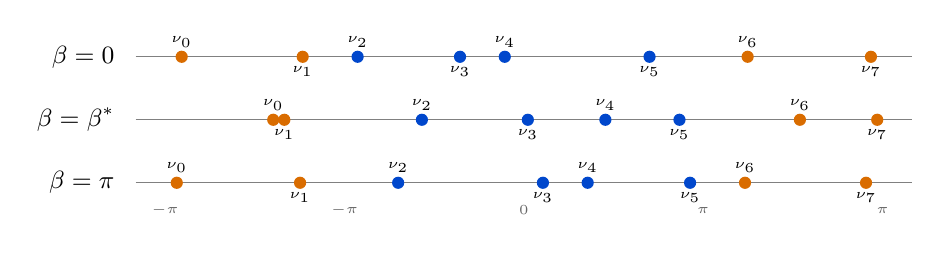
\begin{tikzpicture}[x=1.45cm, y=1cm]
\draw[black!50] (-3.4,1.6) -- (3.4,1.6);
\node[anchor=east,font=\small] at (-3.5,1.6) {$\beta=0$};
\fill[cout] (-2.997,1.6) circle (2.2pt);
\node[font=\tiny,above] at (-2.997,1.6) {$\nu_0$};
\fill[cout] (-1.937,1.6) circle (2.2pt);
\node[font=\tiny,below] at (-1.937,1.6) {$\nu_1$};
\fill[cmid] (-1.456,1.6) circle (2.2pt);
\node[font=\tiny,above] at (-1.456,1.6) {$\nu_2$};
\fill[cmid] (-0.559,1.6) circle (2.2pt);
\node[font=\tiny,below] at (-0.559,1.6) {$\nu_3$};
\fill[cmid] (-0.167,1.6) circle (2.2pt);
\node[font=\tiny,above] at (-0.167,1.6) {$\nu_4$};
\fill[cmid] (1.101,1.6) circle (2.2pt);
\node[font=\tiny,below] at (1.101,1.6) {$\nu_5$};
\fill[cout] (1.960,1.6) circle (2.2pt);
\node[font=\tiny,above] at (1.960,1.6) {$\nu_6$};
\fill[cout] (3.040,1.6) circle (2.2pt);
\node[font=\tiny,below] at (3.040,1.6) {$\nu_7$};
\draw[black!50] (-3.4,0.8) -- (3.4,0.8);
\node[anchor=east,font=\small] at (-3.5,0.8) {$\beta=\beta^\ast$};
\fill[cout] (-2.195,0.8) circle (2.2pt);
\node[font=\tiny,above] at (-2.195,0.8) {$\nu_0$};
\fill[cout] (-2.098,0.8) circle (2.2pt);
\node[font=\tiny,below] at (-2.098,0.8) {$\nu_1$};
\fill[cmid] (-0.893,0.8) circle (2.2pt);
\node[font=\tiny,above] at (-0.893,0.8) {$\nu_2$};
\fill[cmid] (0.035,0.8) circle (2.2pt);
\node[font=\tiny,below] at (0.035,0.8) {$\nu_3$};
\fill[cmid] (0.714,0.8) circle (2.2pt);
\node[font=\tiny,above] at (0.714,0.8) {$\nu_4$};
\fill[cmid] (1.363,0.8) circle (2.2pt);
\node[font=\tiny,below] at (1.363,0.8) {$\nu_5$};
\fill[cout] (2.418,0.8) circle (2.2pt);
\node[font=\tiny,above] at (2.418,0.8) {$\nu_6$};
\fill[cout] (3.095,0.8) circle (2.2pt);
\node[font=\tiny,below] at (3.095,0.8) {$\nu_7$};
\draw[black!50] (-3.4,0) -- (3.4,0);
\node[anchor=east,font=\small] at (-3.5,0) {$\beta=\pi$};
\fill[cout] (-3.040,0) circle (2.2pt);
\node[font=\tiny,above] at (-3.040,0) {$\nu_0$};
\fill[cout] (-1.960,0) circle (2.2pt);
\node[font=\tiny,below] at (-1.960,0) {$\nu_1$};
\fill[cmid] (-1.101,0) circle (2.2pt);
\node[font=\tiny,above] at (-1.101,0) {$\nu_2$};
\fill[cmid] (0.167,0) circle (2.2pt);
\node[font=\tiny,below] at (0.167,0) {$\nu_3$};
\fill[cmid] (0.559,0) circle (2.2pt);
\node[font=\tiny,above] at (0.559,0) {$\nu_4$};
\fill[cmid] (1.456,0) circle (2.2pt);
\node[font=\tiny,below] at (1.456,0) {$\nu_5$};
\fill[cout] (1.937,0) circle (2.2pt);
\node[font=\tiny,above] at (1.937,0) {$\nu_6$};
\fill[cout] (2.997,0) circle (2.2pt);
\node[font=\tiny,below] at (2.997,0) {$\nu_7$};
\foreach \v/\l in {-3.1416/-\pi, -1.5708/-\pi/2, 0/0, 1.5708/\pi/2, 3.1416/\pi}
  \node[font=\tiny, black!60] at (\v,-0.35) {$\l$};
\end{tikzpicture}\\[2pt]
{\small (b) the list at the two ends and at the root}
\caption{Choosing $\beta$. (a)~The eight lifted eigenphases of $C(\beta)$; the middle half $S$ is
blue. Each curve stays continuous because the lift is pinned to the total phase $\sigma(\beta)$.
(b)~At $\beta=\pi$ the list is the mirror image of the list at $\beta=0$, with indices reversed,
so blue stays blue and orange stays orange. At $\beta^\ast$ the blue and orange sums are equal.
(c)~$P$ starts at $P(0)$ and ends at $-P(0)$; bisection homes in on $\beta^\ast$ in a few dozen
evaluations, each one eigendecomposition.}
\label{fig:beta}
\end{figure}

\section*{5. The balanced split at $\beta^\ast$}

At $\beta^\ast$ the four blue phases and the four orange phases have the same sum,
$1.21922$ and $1.21922$. Placing the blue phases on the half
$j_{n-2}=0$ ($+1$ entries of $\mathbf h$) and the orange phases on $j_{n-2}=1$, with
$\theta_j=\nu_j(\beta^\ast)$ and no further branch shift, gives $\varphi=0$
(Fig.~\ref{fig:result}). The pivot $g=R_z(\alpha)R_y(\beta^\ast)$ therefore lets the left-side
multiplexor merge its last two CX gates into the central factor.

\begin{figure}[H]
\centering
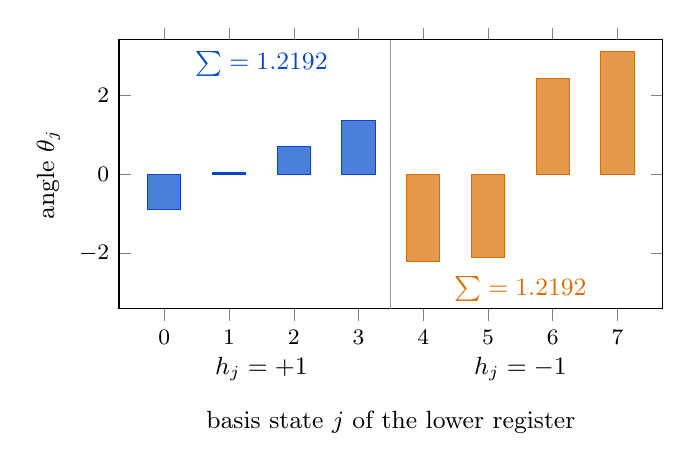
\begin{tikzpicture}
\begin{axis}[ybar, bar width=12pt, bar shift=0pt, width=0.7\textwidth, height=5cm, xmin=-0.7, xmax=7.7,
  xtick={0,...,7}, xlabel={basis state $j$ of the lower register},
  ylabel={angle $\theta_j$}, extra x ticks={1.5,5.5}, extra x tick labels={$h_j=+1$, $h_j=-1$},
  extra x tick style={tick label style={yshift=-14pt, font=\small}, major tick length=0pt},
  ymin=-3.4, ymax=3.4]
\addplot[fill=cmid!70, draw=cmid] coordinates {(0,-0.8933) (1,0.0349) (2,0.7142) (3,1.3634)};
\addplot[fill=cout!70, draw=cout] coordinates {(4,-2.1953) (5,-2.0985) (6,2.4182) (7,3.0947)};
\draw[black!40] (axis cs:3.5,-3.4) -- (axis cs:3.5,3.4);
\node[font=\small, text=cmid] at (axis cs:1.5,2.8) {$\sum=1.2192$};
\node[font=\small, text=cout] at (axis cs:5.5,-2.9) {$\sum=1.2192$};
\end{axis}
\end{tikzpicture}
\caption{The balanced split at $\beta^\ast$. The middle half (blue) is placed on the $+1$ entries
of $\mathbf h$ and the outer quarters (orange) on the $-1$ entries. The two groups have equal
sums, so $\varphi=\frac1D\mathbf h^{\mathsf T}\boldsymbol\theta=0$ and $R_z(\varphi)$ drops out.}
\label{fig:result}
\end{figure}

\end{document}
